%% ------------------------------------------------------- %%
%% SMT-LIB 2.0                                             
%% ------------------------------------------------------- %%
\section{SMT-LIB 2.0}
\subsection{SMT-LIB 2.0 vs SMT-LIB 1.2}
The steps engaged to set up Version 2.0 have consisted in setting up a concrete syntax simpler and leaner than Version 1.2.
The two major additions are the following:
\begin{itemize}
\item A mechanism that approximates parametric sorts and polymorphic function symbols in theory declarations.
\item A command language :
\begin{itemize}
\item to allow user to assert and retract formulas incrementally,
\item to define new sort and function symbols
\item to check the satisfiability of the asserted formulas and query their found model or unsatisfiable core.
\end{itemize}
\end{itemize}


\begin{figure}
\centering
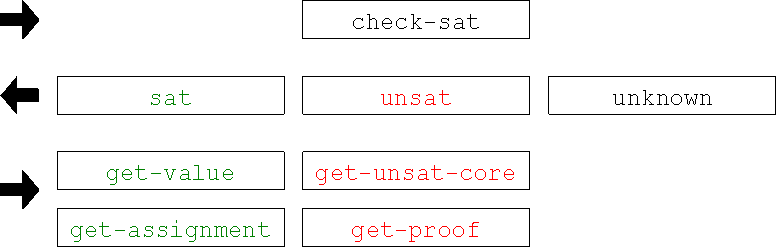
\includegraphics[scale=0.5]{SMT20.png}
\caption{SMT-LIB 2.0 Script Commands} 
\label{Fig:SMT-LIB 2.0}
\end{figure}

\subsection{Solvers' Proof Format}
The commands \textit{get-model} and \textit{get-proof} introduced in SMT-lib v2.0 will be interesting to expose model or counterexample in Rodin. But nowadays, the proof format has not been defined yet in the SMT-Lib v2.0. The Deliverable 7 of DECERT (Task 4:Preliminary Report on a Generic Proof Format for SMT Solvers) will make it clearer and so the integration in Rodin will be possible. 
 
\section{From Event-B to SMT-LIB 2.0}

\subsection{From Event-B AST to SMT-LIB v2.0 AST}
The translation from the Event-B Abstract Syntax Tree (AST) to an SMT-LIB AST V2.0 is very similar to the one to SMT-LIB v1.2 and will not defined again(TODO refer to the previous AST 1.2).

\subsection{From Event-B sequents to benchmarks}
The SMT-LIB parser/checker version 3.0 (\url{http://www.cs.uiowa.edu/~astump/software/ocaml-smt2.zip}) has been used to validate the format of the produced benchmarks.

\paragraph{Assertion}
There is no longer \textbf{assumption} and \textbf{formula} to refer to hypotheses and goal of a sequent. Each hypothesis or goal can be mapped with a benchmark \textbf{assert}. 

\paragraph{Typing Environment}
The typing environment is to be matched to benchmarks \textbf{declare-sort},  \textbf{declare-fun} and/or \textbf{assert}. The following rules apply for the typing environment $\{t \mapsto T\}$, where identifier $t$ has type $T$:
\begin{itemize}
\item If $T$ is the $\intg$ predefined type of the Event-B 
mathematical language, the typing environment is represented 
with the $(declare-fun~t~()~Int)$  SMT-LIB declaration.
\item If $T$ is the $\Bool$ predefined type, it is
represented with the $(declare-fun~t~()~Bool)$  declaration.
\item If $T$ is a user-defined basic type, it is represented
with the $(declare-fun~t~()~T)$ declaration.
\item If $T$ is a cartesian product of two basic types, i.e.\
$T = T_1~\cprod~T_2$, where $T_1$ and $T_2$ are basic types,
and $t~=~(t_1~\mapsto~t_2)$, it is represented with the 
$(declare-fun~t~(T2)~T1)$ declaration.
%% 
%%\item If $T$ is a power-set of a basic type, i.e.\
%%$T~=~\pow(S)$, where $S$ is a basic type, it is represented 
%%with the $(declare-fun~t~()~S)$ declaration, !BEGIN TODO and with an
%%additional assumption: $t \subseteq S$ (see the low-level
%%specification for the expected SMT-LIB syntax for this 
%%assumption) !END TODO.
%%\item If $T$ is a power-set of a cartesian product, i.e.\
%%$T~=~\pow(T_1~\cprod~T_2)$, where $T_1$ and $T_2$ are basic
%%types, it is represented with the !BEGIN TODO $:extrafuns~((t~T_1~T_2))$ 
%%or the $:extrapreds~((t~T_1~T_2))$ declaration. The former
%%is used if $t$ is a function, and the latter if $t$ is a 
%%relation !END TODO.
\end{itemize}

Thus, QF\_LIA is for example the logic for unquantified integer linear arithmetic (i.e.\ boolean combinations of inequations between linear polynomials over integer variables). It refers to the Ints theory.

The linear\_order\_int and linear\_arith theories described in the taxonomy\cite{TAXO09} are to be matched to this logic. 

\paragraph{Example}
For example, if the goal for a sequent is $0 < n + 1$, under the hypothesis $n \in \nat$, in the $\{n \mapsto \intg\}$ typing environment, the associated benchmark is structured as detailed below:
\begin{align*}           
&(set-logic~QF\_LIA)                     \\
&(declare-fun~n~()~Int)                 \\
&(assert~(>~n~0))						\\
&(assert~(>~(+~n~1)~0))					\\
&(check-sat)
\end{align*}


\subsection{Targeted SMT solvers}
For the moment, not every SMT solver supports SMT-Lib 2.0. During the SMT-COMP 2010, many solvers have been introduced to confront each other with SMT v2.0 benchmarks (\url{http://www.smtexec.org/exec/competitors2010.php}). Some of them only parse the 2.0 language and do not include every SMT-Lib 2.0 requirements. Here is an outlook of interesting solvers regarding SMT-lib 2.0:

\begin{itemize}
\item CVC3 \cite{CVC3}(during SMT competition, CVC3 was candidate in those following logics :$UFLRA$, $QF\_UF$, $QF\_RDL$, $QF\_IDL$, $QF\_BV$, $QF\_UFIDL$, $QF\_AX$, $AUFLIA+p$, $AUFLIA-p$, $AUFLIRA$, $QF\_AUFLIA$, $QF\_UFLRA$, $QF\_UFLIA$, $QF\_LRA$, $AUFNIRA$, $UFNIA$, $UFNIA+p$, $QF\_LIA$, $QF\_NIA$, $QF\_UFNRA$, $QF\_NRA$, $QF\_ABV$). 

\item MathSAT 5 \cite{MATHSAT} (during SMT competition, MathSAT was candidate in those following logics : $QF\_UF$, $QF\_UFLRA$, $QF\_UFLIA$, $QF\_LRA$, $QF\_LIA$).

\item OpenSmt \cite{OPENSMT}(during SMT competition, OpenSmt was candidate in those following logics : $QF\_UF$, $QF\_RDL$, $QF\_IDL$, $QF\_UFIDL$, $QF\_LRA$).

\item VeriT\cite{VERIT} (during SMT competition, VeriT was candidate in those following logics : $QF\_UF$, $QF\_RDL$, $QF\_IDL$, $QF\_UFIDL$).

\item Z3 \cite{Z3} (does not take part in SMT competition). 

\end{itemize}

Those solvers parse SMT-Lib 2.0 but not do not support in general unsat core or model generation yet. Only Z3 offers an unsatisfiable core generation via the smt command \textit{(get-unsat-core)}.